%\chapter{Les apports de la visualisation dans l'exploration d'un modèle}
%\label{chap:chap6}
%\begin{center}
%	{\large Version 2018-XX-XX}
%\end{center}
%\minitoc
%
%\section{Comment visualiser des données de simulation?}
%\subsection{Intégrer les données continuellement pour favoriser les allers-retours}
%\subsection{Visualisation et agrégation}
%\subsection{Quelle(s) agrégation(s) d'un espace théorique ?}
%\subsection{Visualiser les variations}
%
%\section{De la visualisation à l'exploration interactive}
%\subsection{Les apports des \textit{visual analytics} à la compréhension des données}
%\subsection{Rendre plus accessibles des données complexes et massives}
%\subsection{Pousser à la sérendipité par l'exploration interactive et intuitive}
%
%\section{Co-évolution du modèle et de ses interfaces d'exploration}
%\subsection{Adapter les outils aux demandes des utilisateurs}
%\subsection{Adapter les outils aux évolutions du modèle}
%\subsection{Comment comparer des modèles dotés d'indicateurs différents ?}


\chapter{Exploration du comportement de SimFeodal}
\label{chap:chap6}
\begin{center}
	{\large Version \hl{2019-08-16}}
\end{center}
\minitoc

\clearpage
\section*{Introduction}
\addcontentsline{toc}{section}{\protect\numberline{}Introduction}

Les chapitres précédents ont présenté le modèle SimFeodal (\hl{chapitre 2}), la manière de l'évaluer (\hl{chapitre 3}), la méthode suivie pour le paramétrage du modèle (\hl{chapitre 4}) et les outils développés pour mener à bien ces étapes de construction et d'évaluation (\hl{chapitre 5}).
Avec cet outillage, théorique, méthodologique et technique, nous sommes désormais en mesure d'explorer le modèle SimFeodal.
Par \og explorer le modèle\fg{}, on entend ici l'exploration des sorties produites par le modèle, sous toutes leurs formes, afin de gagner en connaissance sur ce qui est modélisé, mais aussi sur la manière dont le modèle est construit et implémenté.
Il s'agit autant d'analyser les \og résultats\fg{} de SimFeodal que d'en explorer le fonctionnement et la robustesse.
Ce chapitre est construit en trois parties, assez indépendantes les unes des autres, mais qui se concentrent sur différents aspects de l'évaluation d'un modèle.

La première partie concerne l'analyse des \og résultats\fg{} de SimFeodal, c'est-à-dire les réponses produites par le modèle aux questionnements énumérés dans le \hl{chapitre 3} :
le modèle aboutit-il bien à une polarisation des foyers paysans ?
Le système de peuplement généré par le modèle est-il hiérarchisé tel qu'on l'attendait, et sa distribution est-elle proche des connaissances empiriques ?
Observe-t-on une fixation du peuplement, dans un espace plus disséminé que dans les configurations initiales ?
Pour répondre à ces questions, on présente les étapes de calibrage qui ont permis d'aboutir à une version \og définitive\fg{} du modèle, ainsi que les éléments les plus marquants des indicateurs de sortie issus de cette version.

La deuxième partie de ce chapitre s'attachera à une exploration du comportement en lui-même, c'est-à-dire à sa sensibilité.
Cette sensibilité peut être entendue au sens de robustesse du modèle face aux différentes valeurs de paramètres (analyse de sensibilité classique).
Dans le cas de SimFeodal, une analyse de ce type pose toutefois des questions méthodologiques complexes, en raison notamment du grand nombre de paramètres impliqués et de \og l'explosion combinatoire\fg{} qui en découle.
Un autre perspective sur la sensibilité du modèle concerne sa robustesse face à l'aléa : dans quelle mesure les différents paramètres -- et leurs valeurs associées -- jouent-ils sur la variabilité des indicateurs de sortie ?

La dernière partie doit aussi permettre de gagner en compréhension du modèle en lui-même, et par cela de ce qui est modélisé.
Il s'agira d'explorer des \og scénarios\fg{}, c'est-à-dire de tester des hypothèses, sous la forme d'ensemble de valeurs de paramètres ayant un sens empirique, pour lesquelles le modèle n'a pas été calibré.
La réaction du modèle à ces scénarios sera l'occasion de comprendre plus profondément le comportement du modèle, mais aussi d'esquisser de premières pistes de réponses sur des questions empiriques que se posent les thématiciens spécialistes de la période étudiée.
Ces scénarios peuvent de plus concourir à l'évaluation du modèle.
Ils agissent comme des méthodes de \og validation croisée\fg{} qualitative : si le modèle donne des résultats satisfaisants sur des éléments pour lesquels il n'a pas été construit, cela contribue à renforcer la vraisemblance des postulats sur lesquels il est conçu.

\section{Calibrage du modèle et premiers résultats}

Dans le chapitre 3 (\cref{sec:evaluer-modele}), on indiquait que SimFeodal s'inscrivait dans la lignée des  modèles dont le but est d'\og assister la construction de théories\fg{}, ou encore \og à utilité de développement\fg{}, c'est-à-dire permettant à des chercheurs d'expliciter et de vérifier la cohérence de leurs hypothèses plutôt qu'à les infirmer ou confirmer.

En tant que tels, les \og résultats\fg{} de SimFeodal ne nous semblent donc pas revêtir d'enjeu confirmatoire majeur : ils sont là pour participer à l'évaluation du modèle, tant sur un plan interne qu'externe (cf. \hl{chap3}), mais ne constituent pas pour autant des éléments objectifs et quantifiables de validation.

Dans cette partie, nous rappelons les objectifs du modèle, nous décrivons les étapes de calibrage qui ont été nécessaires afin d'en approcher, et nous présentons enfin les résultats de la version actuelle (6.5.1) du modèle, c'est-à-dire les indicateurs de sortie de simulation issus de cette version, commentés selon la perspective de leur correspondance aux objectifs.

\subsection{Différencier objectifs contextuels et émergents}

\begin{tcolorbox}[breakable,left=0pt,right=0pt,top=0pt,bottom=0pt,
	colback=yellow!50,colframe=black,width=\dimexpr\textwidth\relax, 
	enlarge left by=0mm, boxsep=5pt,arc=0pt,outer arc=0pt]
\textbf{N.B.} : Toute cette partie 6.1.1 (et sans doute 6.1.2) serait bien plus logiquement située dans le chapitre 4 sur le paramétrage.
Il faudra notamment y mettre à jour la typologie des paramètres, et sans doute amener aussi le distinguo entre objectifs émergents et objectifs contextuels, qui en découle largement.
\end{tcolorbox}

Dans les chapitres précédents, on a présenté de manière extensive les objectifs -- dans tous les sens du terme -- poursuivis par le modèle.
Dans le chapitre \hl{2}, on décrivait l'objectif théorique du modèle, à savoir d'aider à la compréhension des phénomènes de restructuration spatiale du système de peuplement rural entre les IX$^e$ et XIII$^e$ siècles.
Dans le chapitre \hl{3}, on présentait la formalisation, au moyen d'indicateurs de sortie de simulation, des résultats du modèle.
En définissant un ensemble d'objectifs, qualifiés (allures de courbes, ordres de grandeur\ldots) sinon quantifiés (les indicateurs numériques), on esquissait un crible d'évaluation du modèle.

Pourtant, même au sein des indicateurs de sortie de simulation, il est une distinction que l'on a pas encore réalisée : le distinguo entre des indicateurs \og émergents\fg{} et des indicateurs \og contextuels\fg{}.

\begin{itemize}
	\item Les premiers sont les indicateurs les plus classiques en modélisation agent : on s'attache à leur évaluation parce qu'ils sont entièrement générés par la combinaison et l'intrication des mécanismes du modèle.
	Parvenir à obtenir des valeurs proches des connaissances empiriques dans ces modèles est un critère de validation d'un modèle, et donc potentiellement un signe d'acquisition de connaissance thématique ou théorique.
	Par exemple, dans SimFeodal, le taux de foyers paysans dispersés en fin de simulation est un pur indicateur émergent : le modèle n'a nullement été paramétré ou calibré pour lui faire atteindre une certaine valeur, et le taux obtenu donne des éléments d'interprétation thématique sur le modèle.
	\item Les indicateurs contextuels n'apportent aucune connaissance thématique.
	Ils remplissent un rôle de cadrage pour les indicateurs émergents : le modèle est paramétré et calibré pour que ces indicateurs parviennent à un résultat pré-décidé.
	Le calibrage des paramètres associés (c'est-à-dire des paramètres qui ont un impact majeur sur ces indicateurs) permet donc d'obtenir un contexte dans lequel les indicateurs émergents pourront être exploités.
	Pour illustrer ces indicateurs de contexte, on peut prendre l'exemple, dans SimFeodal, du nombre de foyers paysans en fin de simulation : ce nombre est entièrement dépendant de deux paramètres (quantité initiale et taux de croissance), et constitue donc presque un \textit{input}, c'est-à-dire ici un contexte au sein duquel les autres indicateurs s'exprimeront.
\end{itemize}

Le tableau des objectifs présent dans SimEDB (\hl{figure 5.8} du \hl{chapitre 5}) correspond à une partie des indicateurs de sortie (les indicateurs numériques ici) de ces deux types, tel qu'indiqué dans le \cref{tab:objectifs-types}.

\begin{table}[H]
	\centering
	\small
	\resizebox{\textwidth}{!}{%
	{\renewcommand{\arraystretch}{1.2}%
	\begin{tabular}{|p{4.5cm}|p{2.1cm}|p{1.75cm}|p{4.5cm}|}
		\hline
		\textbf{Indicateur de sortie de simulation} & \textbf{Valeur attendue} & \textbf{Type} & \textbf{Dépendances directes} \\ \hline
		\textit{Nombre d'agrégats} & \textit{200} & Émergent & \multicolumn{1}{c|}{--} \\ \hline
		\rowcolor[HTML]{DCDCDC} \textit{Nombre de châteaux} & \textit{50} & Contextuel & probabilités de construction de châteaux (PS et GS) \\ \hline
		\textit{Nombre de gros châteaux} & \textit{10} & Émergent & \multicolumn{1}{c|}{--} \\ \hline
		\rowcolor[HTML]{DCDCDC} \textit{Nombre de seigneurs} & \textit{200} & Contextuel & paramètre~dédié~: (\textsf{objectif\_nombre\_seigneurs}) \\ \hline
		\textit{Nombre d'églises paroissiales} & \textit{300} & Émergent & \multicolumn{1}{c|}{--} \\ \hline
		\textit{Distance moyenne entre églises} & \textit{3 000 m} & Émergent & \multicolumn{1}{c|}{--} \\ \hline
		\textit{Part de foyers paysans isolés} & \textit{20 \%} & Émergent & \multicolumn{1}{c|}{--} \\ \hline
		\textit{Augmentation de la charge fiscale des foyers paysans} & \textit{x 3} & Émergent & \multicolumn{1}{c|}{--} \\ \hline
		\rowcolor[HTML]{DCDCDC} \textit{Nombre de Foyers Paysans} & 50 000 & Contextuel & nombre initial; taux de croissance\\ \hline
		\rowcolor[HTML]{DCDCDC} \textit{Densité de population} & 8 feux/km² & Contextuel & nombre de foyers paysans ; taille du monde \\ \hline
	\end{tabular}}}
	\caption{Les indicateurs de sortie de simulation quantitatifs de SimFeodal.}
	\label{tab:objectifs-types}
\end{table}

Notons que si ces indicateurs ont une cohérence à être présentés ensemble au sein de SimEDB, dans le cas d'un tableau de synthèse dédié à l'exploration des résultats de simulation, leur traitement doit nécessairement être différent en matière d'évaluation du modèle.
Cette distinction nous paraît importante en vue d'aborder le calibrage du modèle.
En effet, étant donné la large quantité de paramètres dans le modèle, dont une combinaison judicieuse peut certainement aboutir à des résultats diamétralement opposés, il était nécessaire de restreindre le nombre de paramètres sur lesquels agir pour calibrer le modèle.
Pour que ce calibrage ne soit pas guidé par une logique tautologique, en contraignant le modèle à produire des résultats attendus, on a choisi de mener le calibrage sur les éléments de contexte et sur les éléments techniques (cf. la typologie du \hl{chapitre 4.}\footnote{
	\hl{Le chapitre 4 est à reprendre, notamment en supprimant la typologie des paramètres commensurables, techniques etc. et en la remplaçant par la typologie utilisée dans le modèle, cf. tableau des paramètres : inputs, paramètres de contexte, paramètres de mécanismes, paramètres techniques.}
}
).

\subsection{Calibrage du modèle}

La phase de calibrage diffère des nombreuses étapes de paramétrage décrites dans le \hl{chapitre 4}.
Il  ne s'agit ainsi plus d'ajuster les mécanismes et paramètres pour obtenir une cohérence d'ensemble plus importante dans la manière dont le modèle réagit, mais de se concentrer sur quelques paramètres et indicateurs de sortie\footnote{
Conceptuellement, paramètres et indicateurs sont très largement différents, situés de part et d'autre de la simulation dans une typologie comme celle de Balci (ref chap 4).
Pourtant, dans le cas de ces éléments de contexte, les paramètres sont étroitement liés, de manière presque déterministe, aux indicateurs de sortie qui en découleront.
Pour \og ajuster\fg{} la valeur d'un indicateur de sortie, on pourra donc tester différents ensembles de valeurs pour le ou les paramètres qui agissent directement sur ces indicateurs.
}, contextuels, dont on va régler finement les valeurs de paramètre afin que le contexte de déroulement des autres mécanismes du modèle soit aussi contrôlé et fidèle aux connaissances expertes que possible.

Le calibrage d'un paramètre peut résulter d'un ajustement issu de simulations, par exemple en trouvant de manière expérimentale une valeur de paramètre qui assurera un écart minimal entre l'indicateur de sortie de simulation visé et sa correspondance empirique.
Le calibrage peut aussi être thématique, par exemple en menant une recherche plus approfondie sur les valeurs que peuvent prendre, thématiquement, certains paramètres du modèle au regard des connaissances expertes sur lesquels ils s'appuient.
Ce second type de calibrage pourrait sembler évident, préalable à une démarche rigoureuse et scientifique, et indispensable à réaliser sur chacun des paramètres d'un modèle, ce qui est d'ailleurs vraisemblablement fait dans la plupart des modèles.
Dans un modèle descriptif, exploratoire et surtout basé sur des dynamiques passées, pourtant, la tâche de recherche précise de valeurs pour des dizaines de paramètres semble irréalisable en dehors de projets de modélisation de très large ampleur, ce qui n'est pas le cas de SimFeodal.

Dans les paragraphes suivant, nous donnons des exemples de paramètres et indicateurs qui ont été calibrées dans les dernières phases de paramétrage du modèle.
Ces exemple reprennent la distinction établie ci-dessus entre les types de calibrages : le calibrage des \textit{inputs} est entièrement thématique, celui des paroisses est mixte, entre thématique et expérimental, et le calibrage des châteaux est purement expérimental, guidé par un objectif thématique pré-défini clair.


\subsubsection*{Inputs}
\paragraph{Taille du monde}

Depuis sa conception (en 2014) jusqu'à la version 5.1 (Novembre 2018) du modèle, on avait choisi de simuler les agents du modèle dans un monde théorique, de forme carrée, de 100 km de côté.
Ces dimensions donnaient au monde l'étendue des grands départements français contemporains (ou des petites régions), et constituaient ainsi l'échelle à laquelle on souhaitait modéliser les phénomènes décrits dans SimFeodal.
Les différentes quantités empiriques relatives à cette dimension y étaient donc fortement liées : population, quantité d'églises, de petites villes etc.
On s'appuyait sur l'exemple de la Touraine historique, mais sans hésiter à inclure quelques éléments du duché d'Anjou voisin s'ils avaient été, à un moment ou à un autre, intégrés à notre région d'étude.

En faisant le choix de caler les dimensions du monde simulé plus fortement sur celles de la Touraine historique, il a fallu en premier lieu revoir à la baisse la taille du monde simulé.
La Touraine historique a ainsi une superficie proche de de 6 200 km², qui est ainsi inférieure de plus d'un tiers à la superficie originellement choisie ($100 \times 100$ km, soit 10 000 km²).
On a donc choisi, pour conserver un aspect carré et théorique, de diminuer la taille des côtés du monde simulé à 80 km, dont seuls 79 sont utilisables dans le cadre du modèle (voir le monde restreint, \hl{chapitre 2}), soit une surface de 6 240 km², équivalente à celle de la Touraine.

Dans SimFeodal, la plupart des mécanismes ont une importante composante spatiale.
Dès lors, avec la diminution de la superficie du monde, il a été nécessaire de modifier une large partie des paramètres techniques et certains paramètres de contexte.
Par exemple, un paramètre technique (\textsf{coef\_redevance}) permet d'ajuster le seuil de satisfaction matérielle des foyers paysans en fonction du nombre de redevances dont ils doivent s'acquitter.
En diminuant la taille du monde, et sans diminuer proportionnellement le nombre ou les surfaces des zones de prélèvement, le nombre de redevances des foyers paysans augmente mécaniquement.

\paragraph{Population}
Le nombre de foyers paysans aurait aussi pu être affecté par la taille du monde, mais on le considère comme un \textit{input} guidé par les connaissances empiriques plus que comme un élément contextuel.
Il nous faut ici pondérer fortement ce recours aux connaissances empiriques : il est extrêmement difficile, sinon vain, de parvenir à une simple estimation de la population d'une région française durant la période étudiée.
On peut avoir des indices sur des ordres de grandeur de population à des moments clés de l'histoire, mais d'une part, ils sont extrêmement incertains, et d'autre part, ces moments clés sont souvent différents des seuils temporels sur lesquels nous nous basons.
Sur la Touraine, l'expertise des archéologues et historiens (ref à EZR + Monique Bourrin) permet par exemple d'avoir une idée de la population au début du XVII$^e$ siècle, mais les différentes sources préalables présentent des écarts majeurs.

Pour SimFeodal, on a repris une hypothèse d'historien, qui semble ne pas faire trop débat dans la communauté.
Cette hypothèse consiste à penser qu'un optimum démographique a été atteint au début du XIII$^e$ siècle, et que la population a alors diminué considérablement.
Les historiens estiment que les populations du XIII$^e$ siècle n'ont été rattrapées qu'au début du XVII$^e$.
Il serait donc possible de considérer les populations à l'issu de la période étudiée comme proches de celles, mieux connues empiriquement, du XVII$^e$ siècle.
On a donc choisit de fixer un objectif de population, en fin de simulation (en 1200), à 50 000 foyers paysans, soit une densité d'environ 8 feu / km², ou encore d'environ 40 habitants/km².

\hl{Mettre aussi nb de villes heritées de l'antiquité}

La population initiale est bien plus difficile à estimer.
Selon les sources\footnote{
	\hl{Voir avec les archéos.}
	Par exemple, dans le nord de la France (Picardie, IdF etc.) :  \og \href{https://www.persee.fr/doc/rnord_0035-2624_1998_num_80_326_2872}{La population du Nord au Moyen Age. I : avant 1384}\fg{} de Alain Derville (1998).
}, certains présentent ainsi le IX$^e$ siècle comme un \og nadir\fg{} démographique (c'est-à-dire un minimum dans l'ensemble du moyen-âge), dont la population aurait été multipliée par plus de 7 pour atteindre son niveau optimal à la fin du XIII$^e$.
Pour d'autres historiens et archéologues, rien ne permet de penser qu'il y ait eu une croissance démographique significative entre ces périodes (\hl{voir avec EZR et SL}).

Dans SimFeodal, nous avons choisi l'hypothèse la plus prudente et qui porte le moins d'implications : considérer que la population est relativement stable entre le début et la fin de la période simulée.
Cette \og hypothèse nulle\fg{} n'a pas d'implication thématique forte ici, et nous permettra par la suite de tester des scénarios où l'on ajoute de la croissance démographique dans le déroulement du modèle (voir \cref{subsec:scenario-croissance}).


\subsubsection*{Paroisses}

Le calibrage des paroisses a aussi demandé un calibrage important, et portant cette fois-ci autant sur des aspects thématiques que méthodologiques.
Dans SimFeodal, il existe deux mécanismes distincts de création ou promotion de paroisses (voir \cref{meca-paroisses} dans le \hl{chapitre 2}) : un mécanisme dédié aux églises paroissiales situées dans des agrégats (les paroisses \og urbaines\fg{}) et un mécanisme pour la promotion de nouvelles paroisses en zone peu dense (les paroisses \og rurales\fg{}).
Ces mécanismes servent à faire émerger, de manière guidée, un maillage paroissial similaire, structurellement, à celui que l'on peut reconstituer à partir des connaissances empiriques.
L'apparition et la densification de ce maillage est une conséquence voulue et encouragée des migrations individuelles des foyers paysans.
De plus, ce maillage influe à son tour sur les futures migrations de ces mêmes foyers paysans : les paroisses sont autant une résultante des changements de structure spatiale qu'une partie de leur explication.

Au sein du modèle, la transformation du maillage paroissial joue ainsi un rôle contextuel, conditionnant les migrations des foyers paysans, et un rôle émergent, que l'on observe à une échelle plus agrégées (densification ou étalement, rythmes de changements etc.)

Pour que le contexte permette la meilleure réalisation des phénomènes émergents, il a été nécessaire de calibrer certaines propriétés structurelles du maillage paroissial.

\paragraph{Paroisses \og rurales\fg{}}

Pour les paroisses \og rurales\fg{}, on se base plutôt sur des aspects thématiques issus de connaissances archéologiques.
On connaît ainsi, au moins pour la fin du XII$^e$ siècle, le nombre et la répartition spatiale de la plupart des paroisses (301 églises selon \textcite[31]{zadora-rio_paroisses_2008}, que l'on extrapole par simplicité en 300 paroisses), qui correspondent majoritairement à des milieux ruraux et qui ont en partie perduré dans le maillage communal actuel.
En terme de répartition spatiale, par soucis de généricité, on peut tirer du semis d'églises de l'Indre-et-Loire féodale des distances d'espacement moyennes entre églises paroissiales\footnote{
	On retrouve ainsi cette estimation dans \textcite[261]{chareille_dynamiques_2008} : \og Entre 900 et 1200, l'augmentation importante du nombre de lieux de cultes attestés par les sources écrites se traduit par une diminution nette de l'espacement observé entre les sites : on passe d'une distance moyenne d'un peu plus de 4 km entre deux églises en 900, à une distance d'environ 2,8 km en 1200.\fg{}
}, que l'on utilise ensuite pour calibrer le modèle.

Pour cela, on a joué sur le mécanismes de création/promotion de paroisses rurales et sur les paramètres associés, de manière à approcher des résultats empiriques.
On a fait varier le paramètre \textsf{seuil\_nb\_paroissiens\_insatisfaits} : diminuer la valeur de ce seuil poussait à la création de plus de paroisses rurales, et l'augmenter limitait le nombre final.
Dans l'état actuel du modèle, le nombre de paroisses rurales est encore trop important au regard des connaissances empiriques (380 au lieu de 300, voir le \vref{tab:results-basique}), mais on n'a pas augmenté le seuil pour des raison thématiques.
Le seuil est fixé à 20 foyers paysans, et thématiquement, on estime que cette quantité pouvait suffire à la création d'une nouvelle paroisse.

\paragraph{Paroisses \og urbaines\fg{}}

On dispose de moins de données empiriques pour les paroisses urbaines que pour les paroisses rurales.
On sait que le nombre de paroisses d'une ville est à peu près corrélé à sa population (mais aussi à l'ancienneté de la ville par exemple).
On estime aussi que dans les plus grosses villes de la région (Tours, Loches\ldots), le nombre de paroisses ne dépasse pas la dizaine.
On ne peut pas reconstituer la hiérarchie du nombre de paroisses par villes en fonction des tailles de celles-ci, mais ces éléments empiriques nous fournissent toutefois des cadres pour le calibrage du modèle.

Dans SimFeodal, un seul paramètre (\textsf{ponderation\_creation\_paroisse\_agregat}) contrôle la création de paroisses au sein des agrégats.
Ce paramètre est un \og paramètre de mécanisme\fg{}, quand bien même sa valeur est assez éloignée de l'empirie : elle définit le seuil de foyers paysans (par paroisse urbaine, c'est-à-dire pondéré par le nombre de paroisses présentes dans l'agrégat) à partir duquel la probabilité de créer une nouvelle paroisse dans l'agrégat atteint 1.
On a procédé par calibrage manuel, en testant différentes valeurs pour ce seuil, tout en restant dans des ordres de grandeur acceptables d'un point de vue empirique (on n'aurait par exemple pas pu placer ce seuil à 10 foyers paysans, ce qui aurait signifié qu'on devait créer des paroisses secondaires dans chaque petit agrégat, soit une paroisse par hameau\ldots).

Une difficulté particulière du calibrage a porté sur une des spécificités du mécanisme : il consiste à pondérer le nombre de paroissiens par le nombre de paroisses de l'agrégat.
Dès lors, la définition des \og paroisses de l'agrégat\fg{} revêt une importance considérable et est difficile à stabiliser : un agrégat qui change légèrement de forme entre deux pas de temps peut \og exclure\fg{} une église paroissiale de son emprise, parfois de quelques dizaines de mètres seulement.
Pour minimiser la modification du paramètre de seuil, on a alors agi sur le critère de définition des paroisses d'un agrégat, en ajustant les distances et mécanismes impliqués.


\subsubsection*{Châteaux}

Le calibrage des châteaux a été bien plus simple d'un point de vue thématique : la documentation est précise quant au nombre et aux périodes d'apparition de ces monuments dans l'espace d'étude, et leur nature massive leur a le plus souvent assuré une forte pérennité, atout rare dans l'étude de monuments anciens.
Dans l'ensemble, on sait que le nombre de châteaux\footnote{
	Comme pour la définition des villes, il y a un débat important en archéologie et en histoire sur la définition de ce qu'est un château. Faut-il y inclure, par exemple, les \textit{castra} antiques ? Les mottes castrales ? Dans le cadre de ce modèle, nous avons considéré les \og châteaux forts\fg{}, par nécessité d'établir un référentiel accessible pour la collaboration entre thématiciens et modélisateurs.
} est très faible, si ce n'est nul, au début de la période.
On voit apparaître des châteaux dès le milieu du X$^e$ siècle, sans doute en réaction au climat de violence qui s'établit à ce moment.
En 1200, on estime\footnote{
	L'approximation ne porte pas sur le nombre concret de châteaux construits au total dans la région, mais sur leur date de construction : on ne peut alors que mener une estimation du nombre de châteaux déjà existants à cette date.
} le nombre de châteaux, en Touraine, à une cinquantaine.

Dans SimFeodal, comme les châteaux apportent une protection nécessaire aux foyers paysans, mais en contre-partie permettent aussi aux seigneurs de prélever des droits supplémentaires, leur quantité a une importance certaine, de manière contextuelle, sur le déroulement des simulations.
Une exigence du paramétrage était que le nombre (et le type) de châteaux soit aussi stable que possible au regard des autres mécanismes du modèle et surtout des variations des autres paramètres.

\paragraph{Nombre de châteaux}

Dans les premières versions du mécanisme, des seuils fixes, dépendant de la puissance des seigneurs et donc techniques, avaient ainsi été définis pour caractériser la probabilité de chaque seigneur de construire un château.
Dès lors que les modifications du modèle ont amené à des changements dans la population des foyers paysans (les scénarios démographiques notamment, voir \cref{subsec:scenario-croissance}), le nombre de châteaux a été fortement impacté.

Afin que ce nombre reste stable, on a donc adapté le mécanisme et introduit de nouveaux paramètres techniques permettant de le contrôler.
La \cref{fig:calibrage-param-chateaux} donne un exemple de test de l'un de ces paramètres (qui définit le nombre de tirages aléatoire qu'un grand seigneur peut réaliser pour éprouver sa probabilité de construire un château).
Ce paramètre ayant une influence visuellement linéaire sur le nombre de châteaux en fin de simulation, on peut identifier dans ce graphique que pour obtenir 50 châteaux en fin de simulation (graphique de gauche), la valeur la plus adaptée du paramètre \textsf{nb\_tirages} est de 3.

\begin{figure}[H]
	\centering
	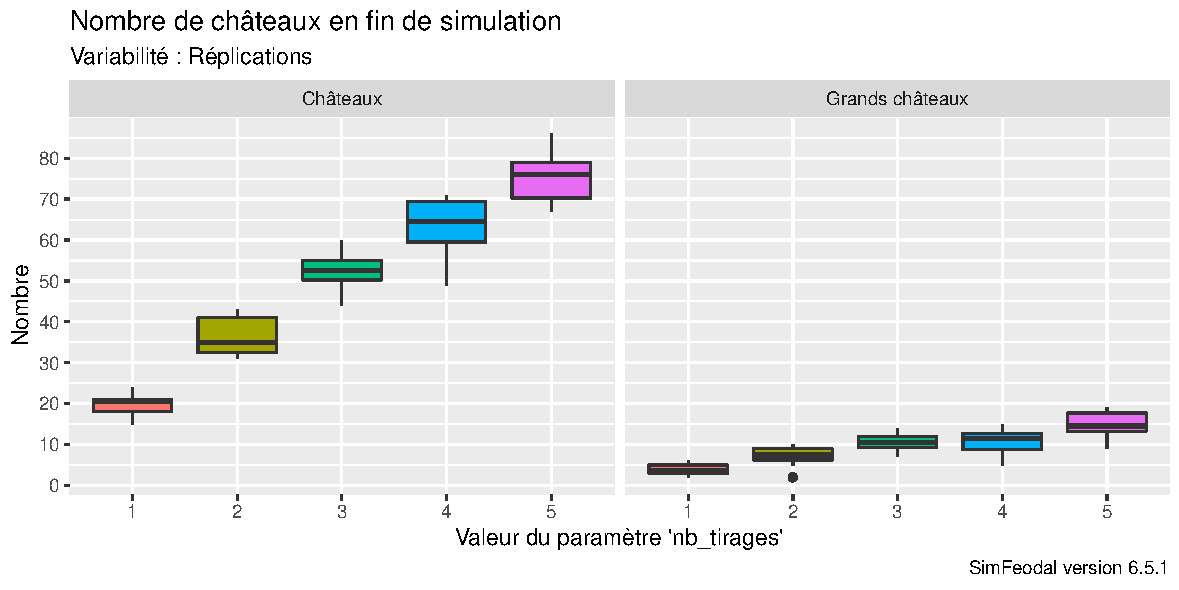
\includegraphics[width=\linewidth]{img/calibrage_nombre_chateaux.pdf}
	\caption[Influence du paramètre \textsf{nb\_tirages} sur le nombre de châteaux.]{Influence du paramètre \textsf{nb\_tirages} sur le nombre de châteaux\footnotemark.}
	\label{fig:calibrage-param-chateaux}
\end{figure}
\footnotetext{
	Ce graphique représente une version légèrement différente de la 6.5.1 présentée dans le reste du chapitre.
	Certaines valeurs de paramètres y sont adaptées au calibrage, fin, des effets de contexte liés aux châteaux.
}

En jouant sur les différents paramètres associés à la construction de château (nombre de tirages et pondérateurs de probabilité pour les grands seigneurs, paramètres liés à la probabilité pour les petits seigneurs\ldots), on parvient à obtenir un résultat relativement stable dans le nombre de châteaux obtenus (\cref{fig:calibrage-chateaux-nb}).

\begin{figure}[H]
	\centering
	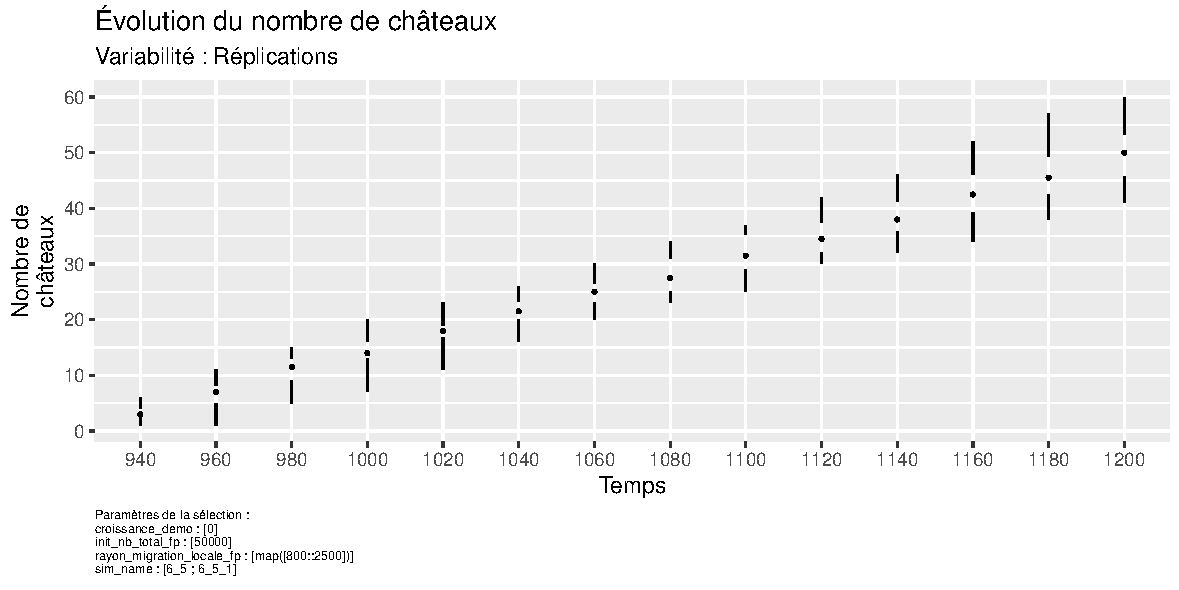
\includegraphics[width=.9\linewidth]{img/results_6_5_1/Chateaux_Nb_Haut.pdf}
	\caption{Évolution du nombre de châteaux après calibration. Version 6.5.1 de SimFeodal.}
	\label{fig:calibrage-chateaux-nb}
\end{figure}

\paragraph{Types et créateurs}

Le nombre de châteaux n'est toutefois pas la seule valeur empirique sur laquelle on essaie d'ajuster le contexte.
On peut ainsi estimer grossièrement la hiérarchie des châteaux, que nous avons choisi de discrétiser entre grands et petits châteaux.
Dans l'ensemble, on estime à une dizaine le nombre de \og grands châteaux\fg{}, c'est-à-dire de \og forteresses\fg{}\footnote{
	Trouver ref. avec Samuel pour distinguer les \og forteresses importantes\fg{} et les \og points fortifiés secondaires\fg{}
}.
On connaît de plus, empiriquement, les seigneurs à l'initiative de la construction des châteaux.
Dans la plupart des cas (de 40 à 45 châteaux), ce sont les seigneurs les plus importants : ducs et comtes d'Anjou et de Touraine, représentés dans SimFeodal par les grands seigneurs.
Les 5 à 10 châteaux restant sont issus de seigneurs de moindre importance qui ont toutefois acquis une puissance symbolique et militaire bien supérieure à celles des autres petits seigneurs.

Pour que le contexte soit correcte en matières de châteaux, il était nécessaire de prendre en compte ces particularités dans le calibrage des mécanismes de création et promotion de château.
Le nombre de châteaux n'était donc pas suffisant, et les paramètres ont du être ajustés afin que ces éléments d'affinage (types des châteaux et types de leurs constructeurs) correspondent aux connaissances empiriques.
Les graphiques de la \cref{fig:calibrage-chateaux-composition} présentent les résultats obtenus dans la dernière version de SimFeodal.
Ils ne sont pas entièrement satisfaisants, mais résultent d'un compromis entre le calibrage des trois indicateurs que sont le nombre, le type et le type de constructeur des châteaux.

\begin{figure}[H]
	\centering
	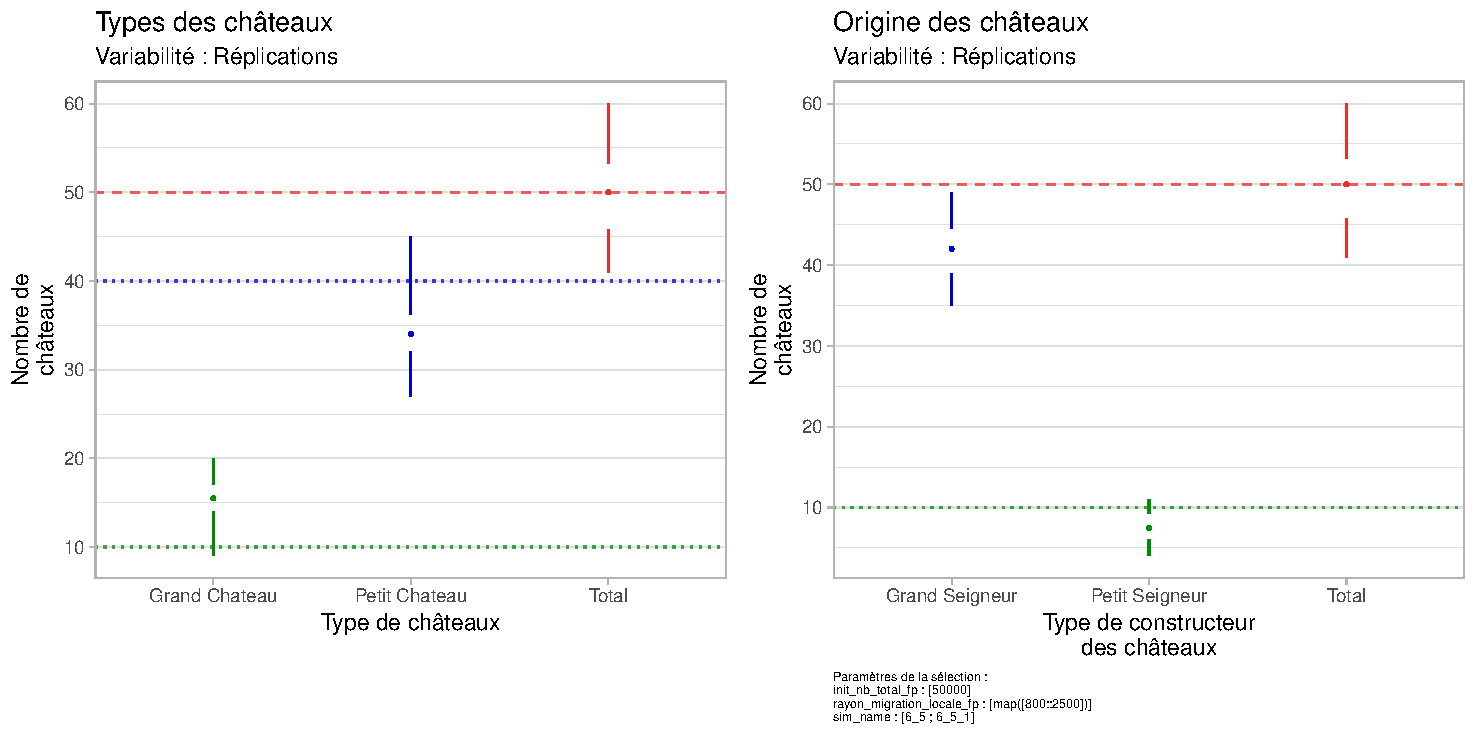
\includegraphics[width=\linewidth]{img/Chateaux_Types_condenses.pdf}
	\caption{Détail de la composition des châteaux en fin de simulation à l'issu du calibrage de SimFeodal.\\
	\textit{Les lignes horizontales en pointillés représentent les objectifs à atteindre.}}
	\label{fig:calibrage-chateaux-composition}
\end{figure}
\end{figure}


\section{Analyser la sensibilité de SimFeodal}
\subsection{Analyse de sensibilité - Méthodo}
\subsection{Analyse de sensibilité - Résultats (quanti))}
\subsection{Analyse de sensibilité - Évaluation visuelle}
\subsection{Analyser la sensibilité à l'aléa}

\section{Comprendre le modèle par l'exécution de scénarios}
\subsection{Tester l'hypothèse d'une croissance démographique}
\subsection{Modéliser la dépendance spatiale : le poids du servage}
\subsection{Quel rôle et importance des communautés paysannes dans la structuration du système de peuplement ?}